%###############################################################################
%# WbXbc - Manual - Bus Splitter                                               #
%###############################################################################
%#    Copyright 2018 Dirk Heisswolf                                            #
%#    This file is part of the WbXbc project.                                  #
%#                                                                             #
%#    WbXbc is free software: you can redistribute it and/or modify            #
%#    it under the terms of the GNU General Public License as published by     #
%#    the Free Software Foundation, either version 3 of the License, or        #
%#    (at your option) any later version.                                      #
%#                                                                             #
%#    WbXbc is distributed in the hope that it will be useful,                 #
%#    but WITHOUT ANY WARRANTY; without even the implied warranty of           #
%#    MERCHANTABILITY or FITNESS FOR A PARTICULAR PURPOSE.  See the            #
%#    GNU General Public License for more details.                             #
%#                                                                             #
%#    You should have received a copy of the GNU General Public License        #
%#    along with WbXbc.  If not, see <http://www.gnu.org/licenses/>.           #
%###############################################################################
%# Version History:                                                            #
%#   September 21, 2018                                                        #
%#      - Initial release                                                      #
%###############################################################################

\subsection[WbXbc Splitter]{WbXbc Splitter (\texttt{WbXbc\_splitter})}
\label{split}

This module implements a bus splitter for the pipelined Wishbone       
protocol. Accesses from the initiator bus are propagated to one of the 
target busses. The target busses are selected by a set of address tags,
generated by the address decoder(see \figref{split:diag}).         
%             +-------------------+             
%             |                   +--->         
% Single      |                   |             
% Initiator   |      WbXbc        +---> Multiple
% Bus     --->|      Splitter     |     Target 
% with        |                   | ... Busses 
% Selects     |                   |             
%             |                   +--->         
%             +-------------------+             
\begin{figure}[!h]
  \begin{center}
    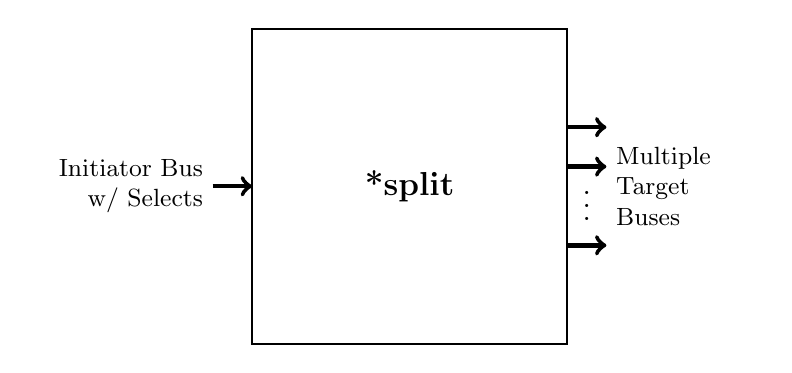
\begin{tikzpicture}
      %Block
      \draw [thick, fill=white] (4,0) rectangle (8,4);
      \node at (6,2)
            {\begin{minipage}[c]{8em}
                \begin{center}
                  \hyphenchar\font=-1
                  \large{\textbf{\nameref*{split}}}
                \end{center}
             \end{minipage}};
      %Inputs     
      \node [left] at (3.5,2)
            {\begin{minipage}[c]{6em}
                \begin{flushright}
                  \hyphenchar\font=-1
                  \small{Initiator Bus w/ Selects}
                \end{flushright}
             \end{minipage}};
      \draw [ultra thick, ->] (3.5,2) -- (4,2);
      %Outputs     
      \node [right] at (8.5,2)
            {\begin{minipage}[c]{5em}
                \begin{flushleft}
                  \hyphenchar\font=-1
                  \small{Multiple Target Buses}
                \end{flushleft}
             \end{minipage}};
      \draw [ultra thick, ->] (8,2.75) -- (8.5,2.75);
      \draw [ultra thick, ->] (8,2.25) -- (8.5,2.25);
      \node [rotate=90] at (8.25,1.75) {\small{\texttt{...}}};
      \draw [ultra thick, ->] (8,1.25) -- (8.5,1.25);
    \end{tikzpicture}
    \caption{Block Diagram of the \nameref*{split}}
    \label{split:diag}
  \end{center}
\end{figure}
  

\subsubsection{Integration Parameters}
\label{split:param}

The \nameref*{split} supports the integration parameters listed in \tabref{split:param:tab}. 
See \secref{param} for a detailed description of all integration parameters.

\begin{center}
  \rowcolors{1}{gray!12}{white}                                         %set alternating row color
  \begin{longtable}{|l|r|l|}
    \rowcolor{white}
    \caption{Integration Parameters of the \nameref*{split}}
    \label{split:param:tab} \\
    %Header
    \hline                                     
    \rowcolor{gray!25}
    \multicolumn{1}{|c|}{\textbf{\rule{0pt}{2.5ex} Parameter}}  &  
    \multicolumn{1}{c|}{\textbf{\rule{0pt}{2.5ex}  Default}}    & 
    \multicolumn{1}{c|}{\textbf{\rule{0pt}{2.5ex}  Decription}} \\
    \hline                                    
    \endhead                               
    %Footers
    \hline
    \rowcolor{white}
    \multicolumn{3}{r}{\tiny{...continued}} \\
    \endfoot
    \hline
    \endlastfoot
    %Content
    \texttt{TGT\_CNT   } & \texttt{4}  & Number of target addresses to decode \\
    \texttt{ADDR\_WIDTH} & \texttt{16} & Width of the address bus             \\
    \texttt{DATA\_WIDTH} & \texttt{16} & Width of each data bus               \\
    \texttt{SEL\_WIDTH } & \texttt{2}  & Number of data select lines          \\
    \texttt{TGA\_WIDTH } & \texttt{1}  & Number of address tags               \\
    \texttt{TGC\_WIDTH } & \texttt{1}  & Number of cycle tags                 \\
    \texttt{TGRD\_WIDTH} & \texttt{1}  & Number of read data tags             \\
    \texttt{TGWD\_WIDTH} & \texttt{1}  & Number of write data tags            \\
  \end{longtable}
\end{center}

\subsubsection{Interface Signals}
\label{split:sig}

\tabref{split:sig:tab} lists the interface signals of the \nameref*{split}. 
See \secref{sig} for a detailed description of all interface signals.

\begin{center}
  \rowcolors{1}{gray!12}{white}                                         %set alternating row color
  \begin{longtable}{|l|r|l|l|}
    \rowcolor{white}
    \caption{Interface Signals of the \nameref*{split}}
    \label{split:sig:tab} \\
    %Header
    \hline                                     
    \rowcolor{gray!25}
    \multicolumn{1}{|c|}{\textbf{\rule{0pt}{2.5ex} Signal}}     &  
    \multicolumn{1}{c|}{\textbf{\rule{0pt}{2.5ex}  Range}}      & 
    \multicolumn{1}{c|}{\textbf{\rule{0pt}{2.5ex}  Direction}}  & 
    \multicolumn{1}{c|}{\textbf{\rule{0pt}{2.5ex}  Decription}} \\
    \hline
    \endhead                               
    %Footers
    \hline
    \rowcolor{white}
    \multicolumn{4}{r}{\tiny{...continued}} \\
    \endfoot
    \hline
    \endlastfoot
    %Section 'Clock and Reset'
    %\hline
    \rowcolor{gray!20}
    \multicolumn{4}{|c|}{\scriptsize{\rule{0pt}{2.5ex} Clock and Reset}} \global\rownum=1\relax \\  
    \hline                                    
    \texttt{clk\_i}        &                                & input & module clock              \\
    \texttt{async\_rst\_i} &                                & input & asynchronous reset        \\
    \texttt{sync\_rst\_i}  &                                & input & synchronous reset         \\
    %Section 'Initiator Interface'
    \hline                                 
    \rowcolor{gray!20}
    \multicolumn{4}{|c|}{\scriptsize{\rule{0pt}{2.5ex} Initiator Interface}} \global\rownum=1\relax \\    
    \hline                                 
    \texttt{itr\_cyc\_i}   &                                & input  & bus cycle indicator       \\
    \texttt{itr\_stb\_i}   &                                & input  & access request            \\
    \texttt{itr\_we\_i}    &                                & input  & write enable              \\
    \texttt{itr\_lock\_i}  &                                & input  & uninterruptable bus cycle \\
    \texttt{itr\_sel\_i}   & \texttt{SEL\_WIDTH-1:0}        & input  & write data selects        \\
    \texttt{itr\_adr\_i}   & \texttt{ADDR\_WIDTH-1:0}       & input  & address bus               \\
    \texttt{itr\_dat\_i}   & \texttt{DATA\_WIDTH-1:0}       & input  & write data bus            \\
    \texttt{itr\_tga\_i}   & \texttt{TGA\_WIDTH-1:0}        & input  & address tags              \\
    \texttt{itr\_tga\_tgtsel\_i} & \texttt{TGT\_CNT-1:0}    & input  & target select tags        \\
    \texttt{itr\_tgc\_i}   & \texttt{TGC\_WIDTH-1:0}        & input  & bus cycle tags            \\
    \texttt{itr\_tgd\_i}   & \texttt{TGWD\_WIDTH-1:0}       & input  & write data tags           \\
    \texttt{itr\_ack\_o}   &                                & output & bus cycle acknowledge     \\
    \texttt{itr\_err\_o}   &                                & output & error indicator           \\
    \texttt{itr\_rty\_o}   &                                & output & retry request             \\
    \texttt{itr\_stall\_o} &                                & output & access delay              \\
    \texttt{itr\_dat\_o}   & \texttt{DATA\_WIDTH-1:0}       & output & read data bus             \\
    \texttt{itr\_tgd\_o}   & \texttt{TGRD\_WIDTH-1:0}       & output & read data tags            \\ 
    %Section 'Target Interface'
    \hline                                                                                      
    \rowcolor{gray!20}
    \multicolumn{4}{|c|}{\scriptsize{\rule{0pt}{2.5ex} Target Interface}} \global\rownum=1\relax \\  
    \hline                                                                                      
    \texttt{tgt\_cyc\_o}         &                          & output & concatinated bus cycle indicators     \\
    \texttt{tgt\_stb\_o}         &                          & output & concatinated access requests	     \\
    \texttt{tgt\_we\_o}          &                          & output & concatinated write enables	     \\
    \texttt{tgt\_lock\_o}        &                          & output & concatinated bus cycle locks	     \\
    \texttt{tgt\_sel\_o}         & \texttt{SEL\_WIDTH-1:0}  & output & concatinated write data selects	     \\
    \texttt{tgt\_adr\_o}         & \texttt{ADDR\_WIDTH-1:0} & output & concatinated write data selects	     \\
    \texttt{tgt\_dat\_o}         & \texttt{DATA\_WIDTH-1:0} & output & concatinated write data busses	     \\
    \texttt{tgt\_tga\_o}         & \texttt{TGA\_WIDTH-1:0}  & output & concatinated address tags	     \\
    \texttt{tgt\_tgc\_o}         & \texttt{TGC\_WIDTH-1:0}  & output & concatinated bus cycle tags	     \\
    \texttt{tgt\_tgd\_o}         & \texttt{TGWD\_WIDTH-1:0} & output & concatinated write data tags	     \\
    \texttt{tgt\_ack\_i}         &                          & input  & concatinated bus cycle acknowledges   \\
    \texttt{tgt\_err\_i}         &                          & input  & concatinated error indicators	     \\
    \texttt{tgt\_rty\_i}         &                          & input  & concatinated retry requests	     \\
    \texttt{tgt\_stall\_i}       &                          & input  & concatinated access delays	     \\
    \texttt{tgt\_dat\_i}         & \texttt{DATA\_WIDTH-1:0} & input  & concatinated read data busses	     \\
    \texttt{tgt\_tgd\_i}         & \texttt{TGRD\_WIDTH-1:0} & input  & concatinated read data tags           \\   
  \end{longtable}
\end{center}  

\subsubsection{Verification Status}
\label{split:verif}

\tabref[Table]{split:verif:tab} provides an overview of the verification status of the \nameref*{split}.
Lint checks have been done with the Icarus Verilog simulator~\cite{iverilog} and the Yosys synthesis tool~\cite{yosys}.

\begin{center}
  \rowcolors{1}{gray!12}{white}                                         %set alternating row color
  \begin{longtable}{|lr|c|c|c|c|}
    \rowcolor{white}
    \caption[Interface Signals]{Verification Status of the \nameref*{split}}
    \label{split:verif:tab} \\
    %Header
    \hline                              
    \rowcolor{gray!25}
    \multicolumn{2}{|c|}{\textbf{\rule{0pt}{2.5ex} Configuration}} &  
    \multicolumn{1}{c|}{\textbf{\rule{0pt}{2.5ex}  Linting}}       &  
    \multicolumn{1}{c|}{\textbf{\rule{0pt}{2.5ex}  Simulation}}    &  
    \multicolumn{1}{c|}{\textbf{\rule{0pt}{2.5ex}  Formal}}        &  
    \multicolumn{1}{c|}{\textbf{\rule{0pt}{2.5ex}  FPGA}}          \\
    \hline                              
    \endhead                               
    %Footers
    \hline
    \rowcolor{white}
    \multicolumn{6}{r}{\tiny{...continued}} \\
    \endfoot
    \hline
    \endlastfoot
    %Content
    \makecell[l]{Default:             \\ 
                 \texttt{ADDR\_WIDTH} \\
                 \texttt{DATA\_WIDTH} \\
                 \texttt{SEL\_WIDTH}  \\
                 \texttt{TGA\_WIDTH}  \\
                 \texttt{TGC\_WIDTH}  \\
                 \texttt{TGRD\_WIDTH} \\
                 \texttt{TGWD\_WIDTH}}   &
    \makecell[r]{                     \\ 
                 \texttt{16}          \\
                 \texttt{16}          \\
                 \texttt{2}           \\
                 \texttt{1}           \\
                 \texttt{1}           \\
                 \texttt{1}           \\
                 \texttt{1}}             &     
    \makecell[c]{iVerilog~\cite{iverilog} \\                    
                 Yosis~\cite{yosys}}     &
    & & \\
  \end{longtable}
\end{center}
  

